\section{Einleitung}
\label{cha:einleitung}
Im Gegensatz zu den vergangenen Jahren war es die Aufgabe dieses Projektseminars Echtzeitsysteme eine Steuerung zu entwickeln, welche einen vorgegebenen Rundkurs durch eine Kamera erkennt und diesen absolvieren kann. In den letzten Jahren wurden Sensoren und die Abstände zu Wänden dafür genutzt. Durch eine Kamera und verschiedene Sensoren wird die Umgebung analysiert und durch Filterung und Regelung umgewandelt, um das Fahrzeug zu steuern. 
Die finale Implementation lässt das Fahrzeug autonom den Rundkurs bewältigen ohne dabei über die markierten Linien zu fahren. Als zweite Aufgabe wurde Hinderniserkennung mit Spurwechsel gewählt, hier erkennt das Fahrzeug ein Hindernis und wechselt die Spur, um diesem auszuweichen. Sollte die Strecke komplett blockiert sein, wird auch dies erkannt und das Fahrzeug hält an.\todo{wenn 2 Hindernisse drin bleibt so lassen, ansonsten raus} \\
In den folgenden Kapiteln werden die Grundlage der Hardware und Software, die Organisation des Teams, die Implementierung der Aufgaben und die Probleme beschrieben.
\todo{Weiter schreiben?}

%%%%%%%%%%%%%%%%%%%%%%%%%%%%%%%%%%%%%%%%%%%%%%%%%%%%%%%%%%%%%%%%%%%%%%%%%%%%%%%%%%%%%%%%%%%%
\clearpage
\section{Grundlagen}
\label{cha:grundlagen}
In diesem Kapitel werden die verschiedenen Grundlagen auf der Hardware- und Softwareseite beschrieben. Dies schließt Informationen über das Modellauto, die verwendeten Kameras, das Metabetriebssystem ROS, OpenCV, die vorgegebenen Packages von PSES und die Gestaltung des Rundkursen in den Veranstaltungsräumen mit ein.

\subsection{Hardware}
\label{sec:hardware}
Die benötigte Hardware für das Projektseminar wurde allen Gruppen zur Verfügung gestellt und es gab eine kurze Einführung in die Arbeitsräume und den Umgang mit den einzelnen Teilen. Zur Verfügung standen das Modellfahrzeug, eine Kinect Kamera, eine Weitwinkelkamera, passende Akkus und Ladestationen und einiges an Klebeband. In den folgenden Unterabschnitten werden das Modellfahrzeug und die Kameras genauer beschrieben. 
\subsubsection{Modellauto}
\label{sec:modellauto}
Das zur Verfügung gesellte Fahrzeug ist einem Auto ähnlich. Es wurde speziell für das Projektseminar entwickelt und durch die TU Darmstadt gepflegt. Es besitzt vier Räder einen Motor und ist mit verschiedenen Sensoren, einer Kamera einem Mini-Computer und Mikrocontrollern ausgestattet. Da sich die Aufgabenstellung dieses Seminars auf Bildverarbeitung fokussierte, wird hier nicht näher auf die anderen Sensoren eingegangen. 
Die Steuerung erfolgt über den Computer, auf welchem ROS läuft (siehe \autoref{sec:ros}). Das Fahrzeug besitzt einen maximalen Lenkwinkel und eine maximale Geschwindigkeit, diese wurden durch eine bereitgestellte Fernsteuerung gemessen.
Das Mainboard ist mit diversen Anschlüssen ausgestattet, die es erlauben eine Tastatur, Maus und einen Bildschirm anzuschließen. Des Weiteren ist eine Kinect und eine Weitwinkelkamera vorhanden (siehe \autoref{sec:kameras}). Die Stromversorgung während der Fahrt übernehmen zwei Akkupacks.
\tod{Bild Auto}
\subsubsection{Kameras}
\label{sec:kameras}
Zu Beginn war eine Kinect Kamera auf dem Fahrzeug verbaut. Diese wurde in den frühen Phasen der Entwicklung genutzt, jedoch kurz nach der Zwischenpräsentation durch die Weitwinkelkamera ersetzt. Diese zeichnet sich durch ein 120° Sichtfeld, eine FullHD Auflösung und einem leicht einstellbaren Positionswinkel aus.
Grund dafür war eine schlechte Farbwahrnehmung der Kinect, diese wurden übersaturiert dargestellt (näheres siehe \autoref{sec:sichtfeld}). Eine Erkennung der richtigen Farbe durch die bereitgestellten Bibliotheken war dadurch nicht mehr möglich. 
Mit der Weitwinkelkamera wurde dieses Problem gelöst. Die Farben wirken natürlicher und sind durch die angewendeten Filtermethoden extrahierbar. Da die Halterung der Webcam auf Computerbildschirme ausgerichtet ist, musste eine elegante Lösung gefunden werden. Ein festkleben mit Klebeband hielt für den Anfang, war jedoch zu anfällig für ein Verstellen der Kamera.
Deswegen  wurde ein 3D-Modell entwickelt und eine passende Halterung im Fablab\footnote{https://www.fablab.tu-darmstadt.de/} gedruckt. Mit dieser konnte die Kamera stabil am Fahrzeug befestigt werden und es gab keine Schwankungen mehr durch andere Kamerapositionen (nähere Informationen in \autoref{sec:befestigung}). 
\begin{figure}
	\centering
	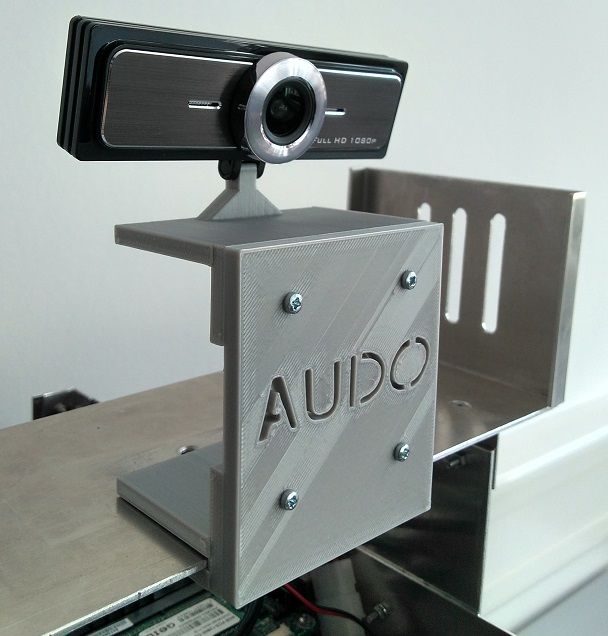
\includegraphics[width=0.5\textwidth]{images/Foto_Halterung.jpg}
	\caption{Halterung der Weitwinkelkamera}
	\label{abb:halterung}
\end{figure}
\tod{Bild updaten}
%%%%%%%%%%%%%%%%%%%%%%%%%%%%%%%%%%%%%%%%%%%%%%%%%%%%%%%%%%%%%%%%%%%%%%%%%%%%%%%%%%%%%%%%%%%%%
\subsection{Software}
\label{sec:software}
In diesem Abschnitt wird die Software vorgestellt, die auf dem Mini-Computer läuft und während der Programmierung genutzt wird. Das Hauptbetriebssystem stellt Lubuntu dar\footnote{https://lubuntu.net/}. Auf diesem ist das Metabetriebssystem ROS installiert, welches die eigentlichen Funktionen übernimmt. Die Programmierung der Nodes geschieht mit dem Programm RoboWare Studio, dort sind alle vorgefertigten Nodes und die selbst erstellten  übersichtlich dargestellt. Programmiert wird in der Programmiersprache C++. \\
Im folgenden werden häufig genutzte Pakete beschrieben und das Meta-Betriebssystem ROS.


\subsubsection{ROS - Robot Operating System}
\label{sec:ros}
ROS ist ein Metabetriebssystem für Roboter, welches auf Linux basiert und in vielen Unternehmen für Steuerung von Robotern genutzt wird. Es stellt mehrere Pakete zur Verfügung, die einige nützliche Funktionen ermöglichen. Dazu gehört die Verteilung auf mehrere Systeme im Netzwerk, Paketverarbeitung und die Kommunikation zwischen den Nodes \cite{einfuehrungROS}.
Die Kommunikation findet durch ein Publish-Subscribe-System statt. Die einzelnen Nodes publishen zu  bestimmten Themen Nachrichten, deren Inhalt sich auf das Thema bezieht. So erhält man zum Thema \code{/uc\_bridge/usr} über eine Subscription Nachrichten über die Werte des rechten Abstandssensors. Auch die Steuerung des Motors und des Lenkwinkels geschieht über das puplishen von Nachrichten. 
Die Eigenschaften der Pakete und Tutorials zu den Funktionen sind auf der Website von ROS zu finden und erleichtern den Einstieg. Durch Open Source lässt sich schnell herausfinden was wirklich benötigt wird und welche Funktionen im späteren Verlauf hilfreich sein könnten.

\subsubsection{OpenCV}
\label{sec:openCV}
Zur Verarbeitung der Kamerabilder wird die freie Bibliothek OpenCV\footnote{https://opencv.org/} genutzt, diese ist auch durch eine Node in ROS eingebunden und einfach nutzbar. Zur Verwendung wird das von der Kamera erhaltene Objekt in der Datenstruktur von OpenCV als \code{cv::Mat} gespeichert. Darauf lassen sich alle späteren Bearbeitungsschritte ausführen. 
Sie stellt viele nützliche Funktionen bereit, die das Erkennen der Fahrspuren und der Hindernisse erleichtern. Dazu gehören zum Beispiel \code{cv::wrapperperspective}, mit der das Bild in eine Bird Eye View umgewandelt wird und \code{cv::imshow} zum Anzeigen des aktuellen Bildes. Interessanterweise funktionierte diese Funktion nur, wenn sie im Zusammenhang mit \code{cv:waitKey} aufgerufen wurde. 
Mittels \code{cv::cvtColor}, \code{cv::inRange} und \code{cv::GaussianBlur} lässt sich der Farbraum des Originalbildes transformieren und in diesem anschließend alle Farben herausfiltern, die in einem bestimmten Bereich liegen. 
In der späteren Verarbeitung war es nötig Farbwerte von einzelnen Pixeln auszuwerten, dies geschah mit Hilfe der Methode \code{cv::mat.at<uchar>(y,x)}. Auch ein Einzeichnen von neuen Punkten war möglich und für die spätere Kurvenerkennung hilfreich. 

\subsubsection{PSES Packages}
\label{sec:psespackages}
Zur Kommunikation mit den einzelnen Fahrzeugteilen sind von den Veranstaltern einige Nodes vorgegeben, dazu gehören \code{pses\_uc\_bridge}, \code{pses\_simulation}, \code{pses\_dashboard} und \code{pses\_odometry}. Von diesen wurde in der finalen Lösung nur \code{pses\_uc\_bridge} genutzt. Diese Node muss zuerst gestartet werden, da sie alle Steuerfunktionen übernimmt und die Publish- und Subscribe-Komponenten für die verschiedenen Werte erstellt. 
Über \code{pses\_dashboard} kann das Fahrzeug manuell gesteuert werden, dies wurde genutzt, um herauszufinden wie groß der maximale Lenkwinkel und die Geschwindigkeit waren, die das Fahrzeug bewältigen kann. Da diese Node gestartet über eine graphische Oberfläche verfügt, war auch ein Ablesen der jeweiligen Sensorwerte möglich. \code{pses\_simulation} stellt eine Simulationsumgebung für das Fahrzeug da, in der der erstellte Code getestet werden konnte. Dies wurde jedoch nicht genutzt, da ein Testen in der realen Umgebung bessere Werte lieferte und in der Simulation kein Kamerabild simuliert werden konnte. 
Die Node \code{pses\_odometry} dient zur Selbstlokalisierung des Fahrzeuges. Nach dem Start ist es möglich die zurückgelegte Strecke und die einzelnen Positionsdatenveränderungen zu berechnen, um sich ein genaueres Bild über die Position des Fahrzeuges in seiner Umwelt zu machen.

%%%%%%%%%%%%%%%%%%%%%%%%%%%%%%%%%%%%%%%%%%%%%%%%%%%%%%%%%%%%%%%%%%%%%%%%%%%%%%%%%%%%%%%%%%%%%%
\subsection{Rundkurs}
\label{sec:rundkurs}
Zur Verfügung standen zwei Räume in Gebäude S311, dort wurden die Fahrzeuge, die Akkus und alles weiter benötigte Material aufbewahrt. Zusätzlich boten sie Platz zum Programmieren und basteln und in einem Raum war der Boden mit einem Rundkurs ausgestattet. Dieser war mit farbigem Klebeband auf eine Teichfolie in mitten des Raumes geklebt. Er bot zwei grüne Linien am Rand und eine pinke Mittellinie. Hier fanden sich öfter mehr als eine Gruppe ein, um den zuvor programmierten Code zu testen, die Kameras einzustellen oder die Lenkwinkel zu messen. \\
Da dieser Rundkurs für die finale Bewertung und den Wettbewerb am Ende genutzt wird, konnte man seine Regelung und Steuerung anpassen und die Lichtverhältnisse konstant halten. Es wurde schnell klar, dass geringe Änderungen des Lichtes eine große Änderung bei der Farbwahrnehmung der Kamera nach sich zogen. 
